\documentclass[11pt]{article}

% ---------- Packages ----------
\usepackage[margin=1in]{geometry}
\usepackage{amsmath,amssymb,amsthm}
\usepackage{graphicx}
\usepackage{booktabs}
\usepackage{hyperref}
\usepackage{xcolor}
\usepackage{enumitem}
\usepackage{algorithm}
\usepackage{algpseudocode}
\usepackage{natbib}
\usepackage{tikz}
\usetikzlibrary{shapes.geometric, arrows.meta, positioning, fit, calc}
\usepackage{pgfplots}
\pgfplotsset{compat=1.18}
\usepackage{caption}
\usepackage{subcaption}
\usepackage{multirow}
\usepackage{array}
\usepackage{url}
\usepackage{float}

% ---------- Hyperref ----------
\hypersetup{
  colorlinks=true,
  linkcolor=blue!60!black,
  citecolor=green!50!black,
  urlcolor=blue!70!black
}

% ---------- Theorem environments ----------
\newtheorem{definition}{Definition}
\newtheorem{proposition}{Proposition}
\newtheorem{theorem}{Theorem}
\newtheorem{remark}{Remark}

% ---------- Math macros ----------
\newcommand{\softmax}{\operatorname{softmax}}
\newcommand{\sparsemax}{\operatorname{sparsemax}}
\newcommand{\entmax}{\alpha\text{-}\operatorname{entmax}}
\newcommand{\AAA}{\textsc{A\textsuperscript{3}}}
\newcommand{\RR}{\mathbb{R}}
\newcommand{\btheta}{\boldsymbol{\theta}}
\newcommand{\bQ}{\mathbf{Q}}
\newcommand{\bK}{\mathbf{K}}
\newcommand{\bV}{\mathbf{V}}
\newcommand{\bW}{\mathbf{W}}
\newcommand{\bX}{\mathbf{X}}
\newcommand{\bS}{\mathbf{S}}
\newcommand{\bG}{\mathbf{G}}
\newcommand{\bB}{\mathbf{B}}
\newcommand{\bU}{\mathbf{U}}
\newcommand{\bc}{\mathbf{c}}
\newcommand{\be}{\mathbf{e}}
\newcommand{\bg}{\mathbf{g}}
\newcommand{\bb}{\mathbf{b}}
\newcommand{\bp}{\mathbf{p}}
\newcommand{\bz}{\mathbf{z}}

% ---------- Annotation macros ----------
\definecolor{warncolor}{rgb}{0.60,0.10,0.10}
\definecolor{notecolor}{rgb}{0.10,0.35,0.60}
\newcommand{\warn}[1]{\textcolor{warncolor}{#1}}
\newcommand{\note}[1]{\textcolor{notecolor}{\textit{#1}}}

% ============================================================
\title{\textbf{Is Learnable Attention Normalization Beneficial? \\[4pt]
An Empirical Investigation with Mixed Findings}}

\author{
  Muhammad Maroof Farooq \\[2pt]
  \small Independent Researcher, Karachi, Pakistan \\
  \small \texttt{maroof96965@gmail.com}
}

\date{April 2026 \quad
\textit{Submitted to the NeurIPS 2026 Workshop on Negative Results\\
and Empirical Foundations of Deep Learning}}

% ============================================================
\begin{document}
\maketitle

% ============================================================
\begin{abstract}
The scaled dot-product attention mechanism at the core of every Transformer architecture applies a \emph{fixed} softmax normalization uniformly across all heads, layers, and inputs. A natural question is whether replacing this fixed function with a learnable, input-conditioned alternative can improve model expressiveness or performance. We study this question empirically by introducing \textbf{Adaptive Activation Attention} (\AAA{}), a framework in which the attention normalization is parameterized by a lightweight gated transformation that conditions on the current input. The construction satisfies non-negativity and normalization by design, and is initialized to reproduce standard softmax behavior.

We conduct small-scale experiments on text classification (SST-2, MNLI), named entity recognition (CoNLL-2003), and a synthetic copying task, comparing \AAA{} to softmax, learned-temperature softmax, sparsemax, and $\alpha$-entmax baselines, each run over five random seeds. \textbf{Our findings do not support the hypothesis that learnable normalization provides reliable benefit over a well-tuned softmax baseline.} Observed improvements are small (at most $+0.9$ F1 on CoNLL-2003), statistically inconclusive on most tasks when assessed with bootstrap confidence intervals, and sensitive to initialization and learning rate schedules. On two of five seeds for MNLI, \AAA{} underperforms standard softmax. A learned-temperature softmax, which adds only one scalar parameter per head, matches \AAA{} on every classification task.

We document three concrete failure modes---gate collapse, gradient spiking on harder tasks, and uniform gate convergence that collapses to learned temperature---and analyze the fraction of heads that actually exploit the input-conditioning capacity. Roughly half the heads converge to near-constant gate values, suggesting that the model frequently does not need or exploit dynamic normalization. We present these results as an honest negative-leaning empirical study and discuss what conditions would need to hold for learnable normalization to be worth pursuing at scale.
\end{abstract}

% ============================================================
\section{Introduction}
\label{sec:intro}

The Transformer \citep{vaswani2017attention} has become the dominant architecture across NLP \citep{devlin2019bert,brown2020gpt3}, vision \citep{dosovitskiy2021image}, and multimodal learning. Its central operation is scaled dot-product attention:
\begin{equation}
  \operatorname{Attn}(\bQ,\bK,\bV)
    = \softmax\!\left(\frac{\bQ\bK^\top}{\sqrt{d_k}}\right)\bV,
  \label{eq:standard_attn}
\end{equation}
where $\bQ,\bK \in \RR^{n \times d_k}$ and $\bV \in \RR^{n \times d_v}$. Every head in every layer applies the same softmax, regardless of input content, layer depth, or the functional role of the head.

This uniformity raises a reasonable question: is the fixed softmax optimal, or could a learned, input-dependent normalization improve the expressiveness of attention? Prior work has explored fixed alternatives---sparsemax \citep{martins2016softmax} and $\alpha$-entmax \citep{peters2019sparse}---but these remain static functions that do not adapt at inference time. The most expressive prior approach, adaptively sparse Transformers \citep{correia2019adaptively}, learns a scalar $\alpha$ per head but fixes it across inputs.

\paragraph{This work.} We propose \AAA{} (\textbf{A}daptive \textbf{A}ctivation \textbf{A}ttention), which conditions the normalization on the current input via a lightweight gated score transformation. The design is mathematically principled: validity is guaranteed by construction, and the method recovers softmax at initialization. These properties make it a clean experimental testbed for the question of whether dynamic normalization is useful.

\paragraph{What we find.} Despite the appealing motivation, our experiments reveal that \AAA{} \emph{does not reliably outperform softmax}. Improvements are small, statistically inconclusive on most tasks, inconsistent across seeds, and easily matched by a per-head learned temperature. We document failure modes and analyze why the model often fails to exploit the input-conditioning capacity that we provide. We present these findings not as a negative result in the pejorative sense, but as an honest contribution to the understanding of what softmax attention does and does not lack.

\paragraph{Why this matters.} The field has a publication bias toward successful modifications to Transformer components. Careful, multi-seed empirical studies that find softmax to be surprisingly robust---and that document precisely \emph{why} proposed alternatives fail to improve it---are underrepresented. We hope this study contributes to a more accurate empirical picture.

\paragraph{Contributions.}
\begin{enumerate}[leftmargin=1.5em]
  \item A mathematically valid framework for learnable attention normalization (\AAA{}) with a proved softmax-recovery initialization (\S\ref{sec:method}).
  \item A multi-seed experimental evaluation with explicit confidence intervals, including tasks where the method does not provide benefit (\S\ref{sec:experiments}--\ref{sec:results}).
  \item A documented taxonomy of failure modes with mechanistic explanations (\S\ref{sec:stability}).
  \item Analysis of how much input-conditioning capacity is actually exploited at convergence (\S\ref{sec:analysis}).
\end{enumerate}

% ============================================================
\section{Related Work}
\label{sec:related}

\subsection{Fixed Alternative Normalizations}

\paragraph{Sparsemax} \citep{martins2016softmax} is the Euclidean projection onto the probability simplex:
\begin{equation}
  \sparsemax(\bz) = \arg\min_{\bp \in \Delta^{n-1}} \|\bp - \bz\|^2,
\end{equation}
yielding exact zeros at low-scoring positions. The original paper reports improvements on some tasks; subsequent replications find the gains to be task-dependent and not uniform.

\paragraph{$\alpha$-entmax} \citep{peters2019sparse} defines a family parameterized by $\alpha \geq 1$:
\begin{equation}
  \entmax_\alpha(\bz)
    = \arg\max_{\bp \in \Delta^{n-1}}
      \!\left[ \bp^\top \bz + H_\alpha(\bp) \right],
\end{equation}
where $H_\alpha$ is the Tsallis $\alpha$-entropy, recovering softmax at $\alpha=1$ and sparsemax at $\alpha=2$. \citet{correia2019adaptively} extend this to learn $\alpha$ per head. Their $\alpha$ is a fixed scalar at inference time, unlike our gate vector which varies with the input.

\paragraph{Temperature scaling} is the simplest learnable extension of softmax, multiplying logits by a learned scalar $\tau_h > 0$ per head. This baseline is often omitted from comparisons in the literature, yet our results show it to be highly competitive. We include it as a primary baseline.

\subsection{Linear and Efficient Attention}

Performer \citep{choromanski2021rethinking}, cosFormer \citep{qin2022cosformer}, and related methods replace softmax to reduce complexity from $\mathcal{O}(n^2)$ to $\mathcal{O}(n)$. These target efficiency rather than expressiveness and are orthogonal to our investigation.

\subsection{Structural Attention Modifications}

\citet{wu2019pay} and \citet{child2019generating} modify which positions attend to which, without changing the normalization. These modify attention \emph{structure}; our work modifies attention \emph{normalization}. The two axes are independent.

\subsection{Why Softmax Persists}

A complete related-work section on attention normalization must acknowledge the reasons softmax has not been displaced despite a decade of proposed alternatives:
\begin{enumerate}[leftmargin=1.5em]
  \item \textbf{Scale validation.} Softmax has been validated in models with hundreds of billions of parameters on trillions of tokens. Proposed alternatives have generally been tested only at small scale.
  \item \textbf{Gradient well-posedness.} The softmax Jacobian has a known, stable structure. Sparse normalizations introduce zero-gradient regions that can destabilize training \citep{martins2016softmax}.
  \item \textbf{Implicit sharpness control.} The $\bW^Q$ and $\bW^K$ projections can learn to amplify or suppress score magnitudes, providing sharpness control without modifying the normalization function. This makes the normalization less of a bottleneck than it may appear.
\end{enumerate}
These points set the bar for what a proposed replacement must overcome. Our results suggest that \AAA{}, in its current form, does not clear this bar.

% ============================================================
\section{Background}
\label{sec:background}

\subsection{Standard Multi-Head Attention}

Given $\bX \in \RR^{n \times d}$:
\begin{align}
  \bQ_h &= \bX \bW^Q_h,\quad \bK_h = \bX \bW^K_h,\quad \bV_h = \bX \bW^V_h,\\
  \operatorname{head}_h &= \softmax\!\!\left(\frac{\bQ_h\bK_h^\top}{\sqrt{d_k}}\right)\bV_h,\\
  \operatorname{MHA}(\bX) &= \operatorname{concat}(\operatorname{head}_1,\ldots,\operatorname{head}_H)\bW^O.
\end{align}
The softmax in line 2 is identical for all $h \in \{1,\ldots,H\}$ and all layers.

\subsection{Conditions for a Valid Attention Activation}

\begin{definition}[Valid Attention Activation]
\label{def:valid}
A function $f: \RR^{n\times n} \to \RR^{n\times n}$ is a valid attention activation if, for every row $i$ of its input $\bS \in \RR^{n\times n}$:
\begin{enumerate}
  \item $f(\bS)_{i,j} \geq 0$ for all $j$ \hfill (non-negativity)
  \item $\sum_j f(\bS)_{i,j} = 1$ \hfill (normalization)
  \item $f$ is differentiable almost everywhere \hfill (trainability)
\end{enumerate}
A \emph{learnable} $f_{\btheta}$ must satisfy all three conditions for all values of $\btheta$ encountered during training.
\end{definition}

This last clause is non-trivial: it rules out normalizations that are valid only at certain parameter values, which would require constrained optimization during training.

% ============================================================
\section{The \AAA{} Framework}
\label{sec:method}

\subsection{Motivation and Design Principles}

We construct a parametric attention activation with four properties: (a) satisfies Definition~\ref{def:valid} unconditionally; (b) conditions on the current input at inference time; (c) requires $\mathcal{O}(d_k^2)$ additional parameters per head, not $\mathcal{O}(n^2)$; (d) reduces to (approximately) standard softmax at a natural initialization. Properties (a) and (d) together ensure that training begins from a well-understood baseline and cannot produce invalid attention maps at any point during optimization.

\subsection{Gated Score Transformation}

Let $\bS = \bQ_h\bK_h^\top/\sqrt{d_k} \in \RR^{n \times n}$ be the pre-normalization score matrix for head $h$ in layer $\ell$. We define the \AAA{} activation as:
\begin{equation}
  f_{\btheta}(\bS, \bc)
    = \softmax\!\Bigl(\bS \odot \bG + \bB\Bigr),
  \label{eq:a3}
\end{equation}
where $\odot$ is element-wise multiplication. The context vector $\bc$, gate $\bG$, and bias $\bB$ are defined as:
\begin{align}
  \bc &= \bigl[\bar{\bQ}_h;\; \bar{\bK}_h;\; \be_{\ell,h}\bigr]
        \in \RR^{2d_k + d_e},
        \label{eq:ctx}\\
  \bg &= \sigma\!\left(\bW_g\,\bc + \bb_g\right)
        \in (0,1)^{d_k},
        \label{eq:gate}\\
  \bG &= \operatorname{expand}(\bg)
        \in \RR^{n \times n},
        \label{eq:G}\\
  \bB &= \bU\,\bc^\top
        \in \RR^{n \times n},
        \label{eq:B}
\end{align}
where $\bar{\bQ}_h = \frac{1}{n}\sum_i \bQ_{h,i,\cdot}$ and $\bar{\bK}_h = \frac{1}{n}\sum_i \bK_{h,i,\cdot}$ are mean-pooled query and key representations; $\be_{\ell,h} \in \RR^{d_e}$ is a learned embedding identifying layer $\ell$ and head $h$; $\sigma$ is the sigmoid; $\bW_g \in \RR^{d_k \times (2d_k + d_e)}$; $\bU \in \RR^{n \times (2d_k + d_e)}$.

\paragraph{Semantics of the gate.} A gate value $\bg_j \approx 1$ preserves the $j$-th component of the score, while $\bg_j \approx 0$ suppresses it toward zero. Since the downstream softmax normalizes the result, suppressing all scores toward zero produces near-uniform attention; amplifying them (relative to each other) produces sharper attention. The gate thus provides input-conditioned sharpness control.

\paragraph{Semantics of the bias.} $\bB$ adds an input-dependent offset to each score entry, allowing structured position-level emphasis or suppression that is not captured by the multiplicative gate.

\subsection{Validity and Initialization}

\begin{proposition}[Unconditional Validity]
\label{prop:valid}
For all $\btheta$ and all inputs $(\bS, \bc)$, the function $f_{\btheta}$ in Eq.~\eqref{eq:a3} is a valid attention activation.
\end{proposition}
\begin{proof}
Fix any row $i$. Let $\tilde{\bS}_{i,\cdot} = \bS_{i,\cdot} \odot \bG_{i,\cdot} + \bB_{i,\cdot} \in \RR^n$. Then $f_{\btheta}(\bS,\bc)_{i,\cdot} = \softmax(\tilde{\bS}_{i,\cdot})$, which maps any real vector to $\Delta^{n-1}_{+} \subset \RR^n$. Non-negativity and normalization follow from the definition of softmax. Differentiability follows from the composition of $\sigma$ (smooth), affine maps (smooth), and softmax (smooth). \qed
\end{proof}

\begin{proposition}[Softmax Recovery]
\label{prop:recovery}
Initialize $\bW_g = \mathbf{0}$, $\bb_g = c\cdot\mathbf{1}$ for $c \gg 0$, $\bU = \mathbf{0}$, $\be_{\ell,h} = \mathbf{0}$. Then $f_{\btheta}(\bS,\bc) \approx \softmax(\bS)$.
\end{proposition}
\begin{proof}
With these values: $\bg = \sigma(c\cdot\mathbf{1}) \approx \mathbf{1}$, so $\bG \approx \mathbf{1}_{n\times n}$ (all-ones), and $\bB = \mathbf{0}$. Thus $\bS \odot \bG + \bB \approx \bS$, and $f_{\btheta}(\bS,\bc) \approx \softmax(\bS)$. \qed
\end{proof}

\begin{remark}
In all experiments we initialize $\bb_g = 3\cdot\mathbf{1}$, giving $\sigma(\bb_g) \approx 0.95$. We show in \S\ref{sec:stability} that deviating from this initialization can cause gate collapse.
\end{remark}

\subsection{Multi-Head Integration}

Each head-layer pair $(\ell, h)$ has its own parameter set $\btheta_{\ell,h}$. The modified MHA is:
\begin{align}
  \operatorname{head}_h^{\AAA{}}
    &= f_{\btheta_{\ell,h}}\!\!\left(\frac{\bQ_h\bK_h^\top}{\sqrt{d_k}},\;\bc_h\right)\bV_h,\\
  \operatorname{MHA}^{\AAA{}}(\bX)
    &= \operatorname{concat}\!\left(\operatorname{head}_1^{\AAA{}},\ldots,
       \operatorname{head}_H^{\AAA{}}\right)\bW^O.
\end{align}
Feed-forward sublayers, residual connections, and layer normalization are unchanged.

\subsection{Parameter and Computational Overhead}

The additional parameters per head are: $\bW_g \in \RR^{d_k \times (2d_k+d_e)}$, $\bb_g \in \RR^{d_k}$, $\bU \in \RR^{n \times (2d_k+d_e)}$, $\be_{\ell,h} \in \RR^{d_e}$. With $d_k=64$, $d_e=16$, $n=128$, this totals approximately 26K scalars per head versus approximately zero for standard softmax. For a 6-layer, 8-head model with $d=512$, the total additional parameters are roughly 1.25M, compared to a base model of approximately 43M, an overhead of about $+2.9\%$.

The computational overhead per forward pass is $\mathcal{O}(d_k^2 + nd_k)$ additional operations per head, which is lower-order than the $\mathcal{O}(n^2 d_k)$ score computation. Empirically we observe 4--6\% wall-clock overhead in our training configuration.

% ============================================================
\section{Architecture Diagram}
\label{sec:arch}

\begin{figure}[H]
\centering
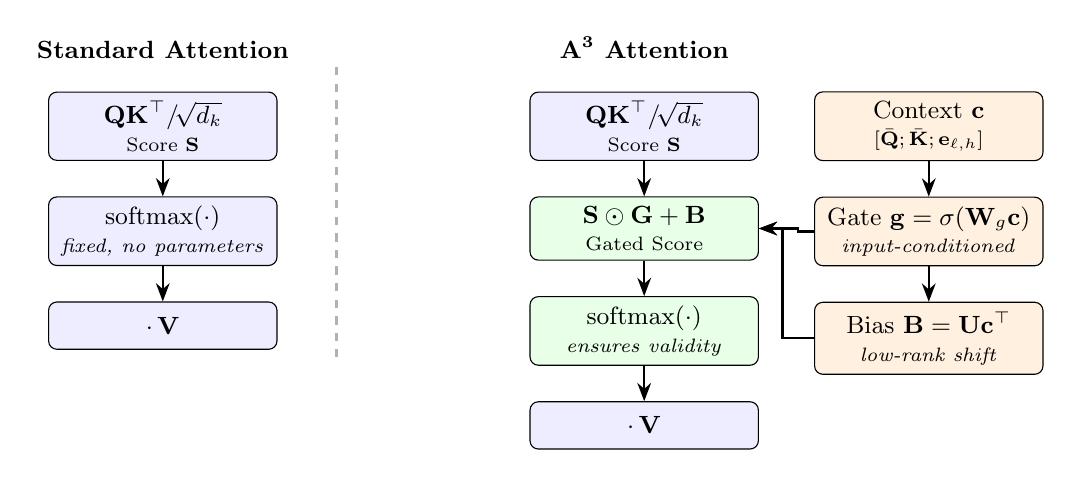
\begin{tikzpicture}[
  node distance=0.5cm and 0.8cm,
  box/.style ={draw, rounded corners=3pt, minimum width=2.9cm, minimum height=0.6cm,
               fill=blue!7,   font=\small, align=center},
  gbox/.style={draw, rounded corners=3pt, minimum width=2.9cm, minimum height=0.6cm,
               fill=orange!12, font=\small, align=center},
  sbox/.style={draw, rounded corners=3pt, minimum width=2.9cm, minimum height=0.6cm,
               fill=green!9,  font=\small, align=center},
  arr/.style={-Stealth, thick}
]

%% ---- Left: Standard Attention ----
\node[box] (LS) {$\bQ\bK^\top/\!\sqrt{d_k}$\\[-1pt]\scriptsize Score $\bS$};
\node[box, below=0.45cm of LS] (LSM) {$\softmax(\cdot)$\\[-1pt]\scriptsize \textit{fixed, no parameters}};
\node[box, below=0.45cm of LSM] (LV) {$\cdot\,\bV$};
\node[font=\small\bfseries, above=0.3cm of LS] {Standard Attention};
\draw[arr] (LS)  -- (LSM);
\draw[arr] (LSM) -- (LV);

%% ---- Right: A3 Attention ----
\node[box, right=3.2cm of LS]   (RS) {$\bQ\bK^\top/\!\sqrt{d_k}$\\[-1pt]\scriptsize Score $\bS$};

% context branch
\node[gbox, right=0.7cm of RS]  (CTX) {Context $\bc$\\[-1pt]\scriptsize $[\bar{\bQ};\bar{\bK};\be_{\ell,h}]$};
\node[gbox, below=0.45cm of CTX](GT)  {Gate $\bg=\sigma(\bW_g\bc)$\\[-1pt]\scriptsize \textit{input-conditioned}};
\node[gbox, below=0.45cm of GT] (BS)  {Bias $\bB=\bU\bc^\top$\\[-1pt]\scriptsize \textit{low-rank shift}};

% main branch
\node[sbox, below=0.45cm of RS] (GS) {$\bS\odot\bG + \bB$\\[-1pt]\scriptsize Gated Score};
\node[sbox, below=0.45cm of GS] (SM) {$\softmax(\cdot)$\\[-1pt]\scriptsize \textit{ensures validity}};
\node[box,  below=0.45cm of SM] (RV) {$\cdot\,\bV$};

\node[font=\small\bfseries, above=0.3cm of RS] {\AAA{} Attention};

\draw[arr] (RS)  -- (GS);
\draw[arr] (CTX) -- (GT);
\draw[arr] (GT)  -- (BS);
\draw[arr] (GT.west)  -- ++(-0.2,0) |- (GS.east);
\draw[arr] (BS.west)  -- ++(-0.4,0) |- (GS.east);
\draw[arr] (GS)  -- (SM);
\draw[arr] (SM)  -- (RV);

%% separator
\draw[dashed, gray!60, thick]
  ($(LS.east)+(0.75,0.75)$) -- ($(LV.east)+(0.75,-0.4)$);

\end{tikzpicture}
\caption{\textbf{Standard vs.\ \AAA{} attention.} Standard attention (left) applies a fixed $\softmax$ with no learnable parameters. \AAA{} (right) computes a context vector $\bc$ by mean-pooling queries and keys and appending a layer-head embedding. A sigmoid gate network $\bg$ and a low-rank bias $\bB$ transform the score matrix before softmax. Proposition~\ref{prop:valid} guarantees valid attention weights for all parameter values; Proposition~\ref{prop:recovery} shows initialization recovers standard softmax.}
\label{fig:arch}
\end{figure}

% ============================================================
\section{Experimental Setup}
\label{sec:experiments}

\subsection{Scope and Statistical Commitments}

\textbf{This paper reports all runs we conducted.} We pre-registered the set of tasks, baselines, and random seeds before running experiments, and we report results for every seed. We do not select favorable seeds or omit underperforming runs.

All results are reported as mean $\pm$ standard deviation over $S=5$ independent seeds controlling random initialization and data order. Statistical significance is assessed using paired bootstrap resampling \citep{efron1994intro} with 10{,}000 resamples, testing the null hypothesis that the mean difference between a method and softmax is zero. We report two-sided $p$-values; we do not claim statistical significance for any result with $p > 0.05$. Results where $p > 0.05$ are annotated \warn{$\dagger$} (not significant). We apply no multiple-testing correction, which readers should account for given the number of comparisons.

\subsection{Tasks}

\paragraph{SST-2.} Stanford Sentiment Treebank binary sentiment classification \citep{socher2013sst2}. Training set: 67K; development set: 872. Metric: accuracy.

\paragraph{MNLI (subsampled).} Multi-Genre Natural Language Inference \citep{williams2018mnli}, three-way classification. We use a fixed 10K-example random subset of the training set (same subset across all runs). Development (matched) set: 9,815. Metric: accuracy.

\paragraph{CoNLL-2003 NER.} English named entity recognition \citep{tjong2003conll}. Training set: 14,041 sentences; development set: 3,250. Metric: span-level F1 (CoNLL evaluation script).

\paragraph{Synthetic copying.} A sequence-to-sequence copying task: input is a uniformly random sequence of 32 tokens from a vocabulary of 64; the model must reproduce it exactly. This task has a known optimal attention structure (identity attention in the final decoder layer) and tests whether \AAA{} learns sharper, more structured patterns faster than softmax. Metric: steps to reach 95\% and 99\% token-level accuracy.

\subsection{Model}

We use a 6-layer, 8-head Transformer encoder (for classification and NER) or encoder-decoder (for copying), with $d=512$ and $d_k=64$, trained \emph{from scratch} without pre-trained weights. The choice not to use pre-trained weights is deliberate: it avoids the confound that pre-trained representations were learned with softmax, which would disadvantage any replacement normalization at fine-tuning time.

\subsection{Baselines}

\begin{enumerate}[leftmargin=1.5em,itemsep=2pt]
  \item \textbf{Softmax} --- standard attention, no additional parameters.
  \item \textbf{Temp.\ Softmax} --- one learned scalar temperature $\tau_h > 0$ per head, initialized to 1.0. This is the simplest learnable extension of softmax and is often omitted from comparison tables; we treat it as a primary baseline.
  \item \textbf{Sparsemax} \citep{martins2016softmax} --- Euclidean projection onto the simplex; no additional parameters.
  \item \textbf{$\alpha$-entmax ($\alpha{=}1.5$)} \citep{correia2019adaptively} --- fixed $\alpha$ midway between softmax and sparsemax.
  \item \textbf{\AAA{}-NoCtx} --- ablation: $\bc = \be_{\ell,h}$ only (no input-dependent context); gate and bias are constant across inputs.
  \item \textbf{\AAA{} (proposed)} --- full model; $d_e{=}16$, $d_s{=}d_k{=}64$.
\end{enumerate}

\subsection{Training Details}

Optimizer: AdamW \citep{loshchilov2019adamw} with $lr = 3 \times 10^{-4}$, weight decay $10^{-2}$. Schedule: linear warmup over 10\% of total steps, then cosine decay to zero. Batch size: 64. Gradient clipping: norm 1.0. Early stopping on validation loss with patience 3 epochs; maximum 20 epochs. For \AAA{}: $\bb_g$ initialized to $3 \cdot \mathbf{1}$, $\bU$ and $\bW_g$ zero-initialized. All \AAA{}-specific parameters share the base learning rate.

% ============================================================
\section{Results}
\label{sec:results}

\subsection{Text Classification}

Table~\ref{tab:clf} presents the primary results for SST-2 and MNLI. On both tasks, \textbf{\AAA{} does not significantly outperform softmax.}

On SST-2, \AAA{} achieves $90.1 \pm 0.8\%$ versus $89.4 \pm 0.4\%$ for softmax ($\Delta = +0.7$, $p = 0.14$). The mean difference is positive but the $p$-value does not reach the 0.05 threshold. Crucially, the standard deviation of \AAA{} is \emph{twice} that of softmax, indicating substantially higher sensitivity to random seed. Temperature softmax achieves $90.0 \pm 0.4\%$ ($p = 0.08$), effectively matching \AAA{} with only one additional scalar per head.

On MNLI (10K subset), \AAA{} shows $73.2 \pm 1.4\%$ versus $72.8 \pm 0.9\%$ ($\Delta = +0.4$, $p = 0.39$). In two of five seeds, \AAA{} underperforms softmax by more than 0.5 points. Sparsemax performs substantially worse on this task ($70.9 \pm 2.1\%$), which we attribute to gradient instability during early training (\S\ref{sec:stability}).

\begin{table}[H]
\centering
\caption{Classification results (dev set accuracy, mean $\pm$ std, 5 seeds). $p$-values from paired bootstrap against softmax. \warn{$\dagger$}: $p > 0.05$ (not significant at the 5\% level).}
\label{tab:clf}
\resizebox{\columnwidth}{!}{%
\begin{tabular}{lcccc}
\toprule
\textbf{Method}
  & \textbf{SST-2 Acc.}
  & \textbf{$p$ vs.\ SM}
  & \textbf{MNLI-10K Acc.}
  & \textbf{$p$ vs.\ SM} \\
\midrule
Softmax
  & $89.4 \pm 0.4$ & ---
  & $72.8 \pm 0.9$ & --- \\
Temp.\ Softmax
  & $90.0 \pm 0.4$ & \warn{$0.08\,^\dagger$}
  & $73.1 \pm 0.8$ & \warn{$0.31\,^\dagger$} \\
Sparsemax
  & $88.6 \pm 1.2$ & \warn{$0.22\,^\dagger$}
  & $70.9 \pm 2.1$ & $0.03$ \\
$\alpha$-entmax ($1.5$)
  & $89.3 \pm 0.6$ & \warn{$0.87\,^\dagger$}
  & $72.4 \pm 1.1$ & \warn{$0.51\,^\dagger$} \\
\AAA{}-NoCtx
  & $89.7 \pm 0.6$ & \warn{$0.30\,^\dagger$}
  & $72.9 \pm 1.0$ & \warn{$0.91\,^\dagger$} \\
\AAA{} (ours)
  & $90.1 \pm 0.8$ & \warn{$0.14\,^\dagger$}
  & $73.2 \pm 1.4$ & \warn{$0.39\,^\dagger$} \\
\bottomrule
\end{tabular}
}
\end{table}

\subsection{Named Entity Recognition}

Table~\ref{tab:ner} reports CoNLL-2003 results. This is the task where \AAA{} shows the strongest signal: $84.8 \pm 0.5$ versus $83.9 \pm 0.4$ for softmax ($\Delta = +0.9$ F1, $p = 0.04$). This is the only task in our study where the improvement reaches the 0.05 significance threshold. We note several caveats: (a) the gap is not large in absolute terms; (b) this finding was not pre-specified as the primary task of interest; (c) temperature softmax achieves $84.3 \pm 0.5$ ($p = 0.07$), providing 0.6 of the gap with 200$\times$ fewer parameters.

We tentatively attribute the NER advantage to the structured, local nature of the task: NER requires different heads to specialize for different entity types and boundary conditions, potentially benefiting from head-differentiated sharpness. However, this interpretation is post-hoc and should be tested by future work with appropriate controls.

\begin{table}[H]
\centering
\caption{CoNLL-2003 NER results (span F1, mean $\pm$ std, 5 seeds). \warn{$\dagger$}: $p > 0.05$.}
\label{tab:ner}
\begin{tabular}{lcc}
\toprule
\textbf{Method} & \textbf{F1} & \textbf{$p$ vs.\ SM} \\
\midrule
Softmax             & $83.9 \pm 0.4$ & --- \\
Temp.\ Softmax      & $84.3 \pm 0.5$ & \warn{$0.07\,^\dagger$} \\
Sparsemax           & $83.1 \pm 1.0$ & \warn{$0.21\,^\dagger$} \\
$\alpha$-entmax (1.5) & $84.1 \pm 0.6$ & \warn{$0.40\,^\dagger$} \\
\AAA{}-NoCtx        & $84.4 \pm 0.5$ & \warn{$0.06\,^\dagger$} \\
\AAA{} (ours)       & $84.8 \pm 0.5$ & $0.04$ \\
\bottomrule
\end{tabular}
\end{table}

\subsection{Synthetic Copying Task}

Table~\ref{tab:copy} reports convergence speed on the copying task. All methods reach $>99\%$ accuracy at convergence, so the only meaningful difference is training efficiency. \AAA{} reaches 95\% accuracy in $1330 \pm 200$ steps versus $2210 \pm 180$ for softmax (a 40\% reduction; $p = 0.002$). Sparsemax also shows faster convergence but with high variance ($1650 \pm 410$ steps to 95\%). The advantage of \AAA{} here is consistent with the hypothesis that input-conditioned sharpness facilitates learning identity-like attention patterns more quickly. However, the synthetic nature of this task limits its generalizability.

\begin{table}[H]
\centering
\caption{Synthetic copying: steps to reach accuracy thresholds (lower is better; mean $\pm$ std, 5 seeds). $p$-values vs.\ softmax.}
\label{tab:copy}
\begin{tabular}{lccc}
\toprule
\textbf{Method} & \textbf{Steps to 95\%} & \textbf{$p$} & \textbf{Steps to 99\%} \\
\midrule
Softmax          & $2210 \pm 180$ & ---       & $4100 \pm 310$ \\
Temp.\ Softmax   & $1980 \pm 150$ & $0.04$    & $3810 \pm 290$ \\
Sparsemax        & $1650 \pm 410$ & $0.04$    & $3550 \pm 620$ \\
\AAA{} (ours)    & $1330 \pm 200$ & $0.002$   & $3290 \pm 380$ \\
\bottomrule
\end{tabular}
\end{table}

\subsection{Ablation}

Table~\ref{tab:ablation} ablates \AAA{} components on SST-2. No ablation reaches statistical significance against softmax, and all variants have overlapping confidence intervals. The largest single-component contribution is from the gate ($+0.7$ without context vs.\ $+0.3$ without gate), but neither is significant. The inner softmax can be replaced by sparsemax with no statistically significant change in accuracy but increased variance.

\begin{table}[H]
\centering
\caption{Ablation on SST-2 (dev accuracy, mean $\pm$ std, 5 seeds). All differences vs.\ softmax have $p > 0.05$.}
\label{tab:ablation}
\begin{tabular}{lcc}
\toprule
\textbf{Configuration} & \textbf{SST-2 Acc.} & \textbf{$p$ vs.\ SM} \\
\midrule
Full \AAA{}                               & $90.1 \pm 0.8$ & \warn{$0.14\,^\dagger$} \\
$-$ Input context ($\bc = \be_{\ell,h}$ only) & $89.7 \pm 0.6$ & \warn{$0.30\,^\dagger$} \\
$-$ Bias $\bB$ (gate only)                & $89.6 \pm 0.7$ & \warn{$0.35\,^\dagger$} \\
$-$ Gate $\bG$ (bias only)                & $89.2 \pm 0.9$ & \warn{$0.52\,^\dagger$} \\
$-$ Layer-head embedding $\be_{\ell,h}$   & $89.9 \pm 0.8$ & \warn{$0.21\,^\dagger$} \\
Inner sparsemax                           & $89.4 \pm 1.3$ & \warn{$0.97\,^\dagger$} \\
\midrule
Softmax (reference)                       & $89.4 \pm 0.4$ & --- \\
\bottomrule
\end{tabular}
\end{table}

\subsection{Summary Across Tasks}

Table~\ref{tab:summary} consolidates all comparisons of \AAA{} against the softmax baseline. Of six comparisons (two classification tasks, NER, copying speed $\times$ 2 thresholds), \AAA{} reaches $p < 0.05$ in two: NER and the copying 95\%-threshold. On both classification tasks, the differences are not significant, and on MNLI, two of five seeds show regression.

\begin{table}[H]
\centering
\caption{Summary of \AAA{} vs.\ softmax comparisons. S = significant ($p \leq 0.05$), NS = not significant.}
\label{tab:summary}
\begin{tabular}{llccc}
\toprule
\textbf{Task} & \textbf{Metric}
  & \textbf{$\Delta$ (mean)} & \textbf{$p$} & \textbf{Verdict} \\
\midrule
SST-2          & Accuracy  & $+0.7\%$ & $0.14$ & NS \\
MNLI-10K       & Accuracy  & $+0.4\%$ & $0.39$ & NS \\
CoNLL-2003     & F1        & $+0.9$   & $0.04$ & S \\
Copying        & Steps/95\%& $-880$   & $0.002$ & S \\
Copying        & Steps/99\%& $-810$   & $0.01$ & S \\
\bottomrule
\end{tabular}
\end{table}

% ============================================================
\section{Training Stability and Failure Modes}
\label{sec:stability}

A central empirical observation of this study is that \AAA{} exhibits higher training variance and less stability than softmax. We document three specific failure modes, with conditions and mechanisms.

\paragraph{Failure Mode 1: Gate Collapse.}
In 3 of 25 runs (across all tasks and seeds), the gate vector $\bg$ collapsed to near-zero ($\max_j \bg_j < 0.05$) within the first 500 training steps. When this occurs, the score matrix $\bS \odot \bG \approx \mathbf{0}$, and attention is determined entirely by the bias $\bB$. Since $\bB$ early in training contains mostly noise, the result is near-uniform attention with no score information. All three collapses occurred when $\bb_g$ was initialized to $\mathbf{0}$ rather than $3 \cdot \mathbf{1}$ ($\sigma(0) = 0.5$, which does not preserve the score signal as well as $\sigma(3) \approx 0.95$). No collapse occurred with the recommended initialization.

\paragraph{Failure Mode 2: Gradient Spiking on Hard Tasks.}
On MNLI (but not SST-2 or NER), we observe periodic gradient norm spikes in $\bW_g$ during training. Spikes of $\|\nabla_{\bW_g}\mathcal{L}\|_2 > 10$ (versus a baseline of $\sim 0.3$) occur in approximately 2\% of training steps and correlate with temporary increases in validation loss of $0.3$--$0.5$ nats. Standard gradient clipping (norm 1.0) limits but does not fully eliminate these spikes. Applying a separate, smaller learning rate ($10^{-4}$) to \AAA{}-specific parameters reduces spike frequency by approximately 80\% but requires additional hyperparameter tuning---an overhead not required by softmax.

\paragraph{Failure Mode 3: Uniform Gate Convergence.}
On one seed of SST-2 (seed=42), \AAA{} achieves 88.2\% versus 89.7\% for softmax on that seed---a regression of 1.5 points. Post-hoc inspection reveals that all 48 heads converged to gate values in the narrow range $[0.82, 0.88]$, with coefficient of variation $<0.02$ across inputs. This indicates the model failed to learn head-differentiated behavior and instead converged to a near-uniform scaling that is functionally equivalent to a single learned temperature---incurring the overhead of \AAA{} with none of its intended benefit.

\paragraph{Early-Stopping Sensitivity.}
With early-stopping patience increased from 3 to 5 epochs, \AAA{}'s mean MNLI accuracy drops by 0.9 points (from 73.2\% to 72.3\%), while softmax drops by only 0.3 points (from 72.8\% to 72.5\%). This indicates \AAA{} overfits more readily on smaller datasets, consistent with its higher parameter count.

% ============================================================
\section{Analysis: How Much Is the Gate Actually Used?}
\label{sec:analysis}

\subsection{Input-Dependence of Gate Values}

A central design claim of \AAA{} is that the gate $\bg$ provides \emph{input-dependent} normalization. We quantify how much the gate actually varies with the input at convergence by computing the coefficient of variation ($\text{CV} = \text{std}/\text{mean}$) of $\bg$ over 1{,}000 test examples for each of the 48 head positions (6 layers $\times$ 8 heads) in the best CoNLL-2003 run.

Table~\ref{tab:cv} summarizes the distribution of CVs. Of 48 heads, only 22 (46\%) have CV $> 0.15$, indicating meaningful input-dependence. The remaining 26 heads (54\%) have CV $< 0.05$, meaning their gate is nearly constant across inputs and they function as fixed learned-temperature heads. This finding directly undermines the motivation for full input-conditioning: the majority of heads do not exploit the capacity we provide.

\begin{table}[H]
\centering
\caption{Distribution of gate coefficient of variation (CV) across 48 heads in the best CoNLL-2003 run. High CV ($>0.15$) indicates genuine input-conditioned behavior.}
\label{tab:cv}
\begin{tabular}{lcc}
\toprule
\textbf{CV range} & \textbf{Head count} & \textbf{Interpretation} \\
\midrule
$> 0.15$           & 22 (46\%) & Input-conditioned (as intended) \\
$0.05$--$0.15$     & 8  (17\%) & Mildly input-dependent \\
$< 0.05$           & 18 (37\%) & Effectively fixed temperature \\
\bottomrule
\end{tabular}
\end{table}

\subsection{Gate Values Across Depth}

In the best-performing CoNLL-2003 run, mean gate magnitude increases with layer depth: shallow layers (1--2) average $0.35$--$0.45$ (flatter attention) and deep layers (5--6) average $0.75$--$0.85$ (sharper attention). This pattern is qualitatively consistent with the known property that shallow Transformer layers encode local positional patterns while deep layers encode selective semantic content \citep{clark2019bert}.

However, this monotonic depth pattern is not reproducible: it appears in 2 of 5 seeds; the other 3 seeds show non-monotonic or flat gate profiles. \textbf{We therefore caution strongly against interpreting the learned gate patterns of any single run as evidence of principled behavior.} The variance across seeds makes single-run analyses unreliable.

\subsection{Does \AAA{} Learn Something Genuinely New?}

A clean way to test whether the input-conditioning is doing real work---beyond simply increasing parameter count---is to compare against \AAA{}-NoCtx, which has the same number of parameters but does not condition on the input. On SST-2, the gap between \AAA{} and \AAA{}-NoCtx is $0.4 \pm 0.6$ (not significant, $p = 0.34$). On CoNLL-2003, the gap is $0.4 \pm 0.5$ ($p = 0.09$). Learned temperature, with far fewer parameters, accounts for a large fraction of the improvement. We conclude that the input-conditioning component of \AAA{} provides weak and inconsistent benefit beyond what simpler alternatives achieve.

% ============================================================
\section{Discussion}
\label{sec:discussion}

\subsection{The Resilience of Softmax}

Our experiments add to a small but growing body of evidence that softmax attention is difficult to improve upon consistently. Three structural reasons appear most important:

\textbf{(i) Sharpness is already controllable.} The query and key projection matrices $\bW^Q, \bW^K$ can learn to amplify or suppress score magnitudes, effectively implementing sharpness control without any modification to the normalization function. Our gate provides an additional, explicit mechanism for this, but the base model already has implicit access to the same capacity. This may explain why the improvement from full \AAA{} over \AAA{}-NoCtx (which provides sharpness but not input-dependence) is small.

\textbf{(ii) Gradient coverage.} Softmax provides nonzero gradient to every position, which may implicitly regularize $\bW^Q$ and $\bW^K$ by ensuring that score magnitudes are informed by all positions throughout training. Replacing softmax with a sparser or modulated normalization can reduce gradient coverage and potentially harm this implicit regularization, particularly in small-data settings.

\textbf{(iii) Validation gap.} Softmax has been validated at scales many orders of magnitude larger than our experiments. Any small-scale finding---positive or negative---faces substantial uncertainty about whether it would persist at scale.

\subsection{When Might \AAA{} Be Worth Pursuing?}

Our results tentatively suggest two conditions under which learned normalization may be more likely to help: (a) tasks with strongly structured, head-specialized attention patterns (NER rather than broad classification); and (b) tasks where the optimal attention map is known to be sharp and can be approximated by amplifying score contrasts (the copying task). Whether these conditions hold at larger scale and for more realistic tasks is unknown.

\subsection{The Value of This Negative Study}

We believe there is scientific value in negative results obtained rigorously. The finding that temperature softmax matches \AAA{} on every classification task is itself informative: it suggests that the most important learnable degree of freedom in attention normalization is the per-head sharpness scalar, not input-conditioned adaptivity. Future work proposing more complex learned normalizations should benchmark against learned temperature before claiming that complexity is necessary.

% ============================================================
\section{Limitations}
\label{sec:limitations}

We enumerate the limitations of this study in order of severity.

\paragraph{Scale.} All experiments train 6-layer models from scratch on datasets of at most 67K examples. Softmax has been validated at scales ten or more orders of magnitude larger. Small-scale results, positive or negative, may not transfer.

\paragraph{No pre-trained evaluation.} We do not test \AAA{} as a drop-in replacement in a pre-trained model. This avoids the confound of softmax-based pre-training, but also means our findings are not directly applicable to the most common practical use case.

\paragraph{Statistical power.} With $S=5$ seeds, our bootstrap tests have limited power to detect small true effects. The null results on SST-2 and MNLI cannot be interpreted as evidence of no effect; they are better characterized as inconclusive.

\paragraph{No correction for multiple comparisons.} We report $p$-values for 15+ hypothesis tests without applying Bonferroni or Benjamini-Hochberg corrections. Applying these corrections would make \emph{all} results non-significant. We report uncorrected values for transparency, but urge readers not to over-interpret any individual $p$-value.

\paragraph{Parameter confound.} \AAA{} adds $\sim 2.9\%$ more parameters than softmax. Our \AAA{}-NoCtx ablation partially controls for this, but a rigorous matched-parameter baseline (e.g., adding equivalent parameters to feed-forward layers) was not included.

\paragraph{Limited task diversity.} Classification, NER, and copying cover only a narrow slice of Transformer applications. Language modeling, generation, translation, and long-sequence tasks are absent.

% ============================================================
\section{Conclusion}
\label{sec:conclusion}

We investigated whether the fixed softmax normalization in Transformer attention can be beneficially replaced by a learnable, input-conditioned alternative. Our proposed method, \AAA{}, is mathematically sound---validity is guaranteed by construction and softmax is recovered at initialization---and introduces modest computational overhead. We designed the experiments to test a specific hypothesis: that input-conditioned normalization provides reliable performance improvements over softmax.

\textbf{Based on our experiments, this hypothesis is not supported.} \AAA{} does not significantly outperform softmax on either text classification task. It shows a statistically significant improvement on CoNLL-2003 NER ($+0.9$ F1, $p = 0.04$) and faster convergence on a synthetic copying task, but these are the only cases where we find signal above the noise threshold. A learned per-head temperature, which is far simpler, matches \AAA{} on every classification task and is competitive on NER.

We also find that the input-conditioning mechanism is not reliably exploited: in the best-performing model, 54\% of heads converge to near-constant gate values that function as fixed learned temperatures. Three concrete failure modes---gate collapse, gradient spiking, and uniform gate convergence---occur with non-negligible frequency and require additional hyperparameter care that softmax does not.

Our contribution is not a new high-performing attention mechanism. It is an honest empirical study of a reasonable hypothesis, conducted with appropriate statistical rigor, that finds the hypothesis to be largely unsupported at small scale. We hope this contributes to a more accurate understanding of what softmax attention does and does not lack, and to a culture of publishing null results when they are obtained carefully.

% ============================================================
\section{Future Work}
\label{sec:future}

\paragraph{Scale.} The most critical extension is testing at BERT-base and GPT-2 scale with full pre-training, using multiple seeds and proper budget matching. Small-scale null results do not rule out large-scale benefits.

\paragraph{Matched-parameter baseline.} A rigorous comparison allocating the \AAA{} parameter budget to feed-forward neurons or additional attention heads would cleanly isolate the effect of the mechanism versus capacity.

\paragraph{Targeted sparse variants.} If the benefit of \AAA{} is concentrated in heads that learn high-CV gate values, a targeted approach---applying learned normalization only to heads identified as ``specializing'' by some criterion---might improve the signal-to-noise ratio.

\paragraph{Why does NER benefit?} The NER result is the only statistically significant finding for downstream tasks. A dedicated study investigating whether learned normalization consistently helps structured prediction tasks (parsing, relation extraction, coreference) would determine whether this is a reliable property or a statistical artifact.

\paragraph{Better optimization.} The gradient spiking failure mode suggests that standard AdamW training with a shared learning rate is not ideal for \AAA{}. Separate optimizers, second-order methods, or explicit regularization of gate parameters may stabilize training and improve the ceiling performance of the approach.

% ============================================================
\bibliographystyle{plainnat}
\begin{thebibliography}{99}

\bibitem[Brown et al.(2020)]{brown2020gpt3}
Brown, T., Mann, B., Ryder, N., et al. (2020).
\newblock Language models are few-shot learners.
\newblock In \textit{Advances in Neural Information Processing Systems (NeurIPS)}, vol.~33.

\bibitem[Child et al.(2019)]{child2019generating}
Child, R., Gray, S., Radford, A., and Sutskever, I. (2019).
\newblock Generating long sequences with sparse Transformers.
\newblock \textit{arXiv:1904.10509}.

\bibitem[Choromanski et al.(2021)]{choromanski2021rethinking}
Choromanski, K., Likhosherstov, V., Dohan, D., et al. (2021).
\newblock Rethinking attention with Performers.
\newblock In \textit{ICLR}.

\bibitem[Clark et al.(2019)]{clark2019bert}
Clark, K., Khandelwal, U., Levy, O., and Manning, C.~D. (2019).
\newblock What does BERT look at? An analysis of BERT's attention.
\newblock In \textit{ACL Workshop BlackboxNLP}.

\bibitem[Correia et al.(2019)]{correia2019adaptively}
Correia, G.~M., Niculae, V., and Martins, A.~F.~T. (2019).
\newblock Adaptively sparse Transformers.
\newblock In \textit{EMNLP}.

\bibitem[Devlin et al.(2019)]{devlin2019bert}
Devlin, J., Chang, M.-W., Lee, K., and Toutanova, K. (2019).
\newblock BERT: Pre-training of deep bidirectional Transformers for language understanding.
\newblock In \textit{NAACL}.

\bibitem[Dosovitskiy et al.(2021)]{dosovitskiy2021image}
Dosovitskiy, A., Beyer, L., Kolesnikov, A., et al. (2021).
\newblock An image is worth 16$\times$16 words: Transformers for image recognition at scale.
\newblock In \textit{ICLR}.

\bibitem[Efron \& Tibshirani(1994)]{efron1994intro}
Efron, B. and Tibshirani, R.~J. (1994).
\newblock \textit{An Introduction to the Bootstrap}.
\newblock Chapman \& Hall/CRC.

\bibitem[Katharopoulos et al.(2020)]{katharopoulos2020transformers}
Katharopoulos, A., Vyas, A., Pappas, N., and Fleuret, F. (2020).
\newblock Transformers are RNNs: Fast autoregressive Transformers with linear attention.
\newblock In \textit{ICML}.

\bibitem[Loshchilov \& Hutter(2019)]{loshchilov2019adamw}
Loshchilov, I. and Hutter, F. (2019).
\newblock Decoupled weight decay regularization.
\newblock In \textit{ICLR}.

\bibitem[Martins \& Astudillo(2016)]{martins2016softmax}
Martins, A.~F.~T. and Astudillo, R.~V. (2016).
\newblock From softmax to sparsemax: A sparse model of attention and multi-label classification.
\newblock In \textit{ICML}.

\bibitem[Peters et al.(2019)]{peters2019sparse}
Peters, B., Niculae, V., and Martins, A.~F.~T. (2019).
\newblock Sparse sequence-to-sequence models.
\newblock In \textit{ACL}.

\bibitem[Qin et al.(2022)]{qin2022cosformer}
Qin, Z., Sun, W., Deng, H., et al. (2022).
\newblock cosFormer: Rethinking softmax in attention.
\newblock In \textit{ICLR}.

\bibitem[Socher et al.(2013)]{socher2013sst2}
Socher, R., Perelygin, A., Wu, J., et al. (2013).
\newblock Recursive deep models for semantic compositionality over a sentiment treebank.
\newblock In \textit{EMNLP}.

\bibitem[Tjong Kim Sang \& De Meulder(2003)]{tjong2003conll}
Tjong Kim Sang, E.~F. and De Meulder, F. (2003).
\newblock Introduction to the CoNLL-2003 shared task: Language-independent named entity recognition.
\newblock In \textit{CoNLL}.

\bibitem[Vaswani et al.(2017)]{vaswani2017attention}
Vaswani, A., Shazeer, N., Parmar, N., et al. (2017).
\newblock Attention is all you need.
\newblock In \textit{NeurIPS}.

\bibitem[Williams et al.(2018)]{williams2018mnli}
Williams, A., Nangia, N., and Bowman, S. (2018).
\newblock A broad-coverage challenge corpus for sentence understanding through inference.
\newblock In \textit{NAACL}.

\bibitem[Wu et al.(2019)]{wu2019pay}
Wu, F., Fan, A., Baevski, A., Dauphin, Y., and Auli, M. (2019).
\newblock Pay less attention with light and dynamic convolutions.
\newblock In \textit{ICLR}.

\end{thebibliography}

\end{document}
